\documentclass{article}

\usepackage[american]{circuitikz}

\begin{document}
    
    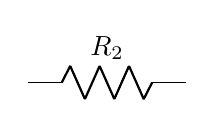
\begin{tikzpicture}
        \draw (0,0) to[R=$R_2$] (2,0);
    \end{tikzpicture}

    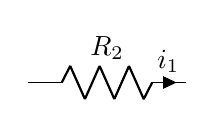
\begin{tikzpicture}
        \draw (0,0) to[R=$R_2$, i=$i_1$] (2,0);
    \end{tikzpicture}
    
    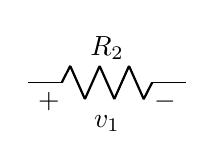
\begin{tikzpicture}
        \draw (0,0) to[R=$R_2$, v=$v_1$] (2,0);
    \end{tikzpicture}

    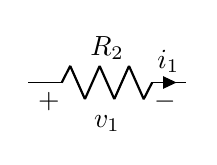
\begin{tikzpicture}
        \draw (0,0) to[R=$R_2$, i=$i_1$, v=$v_1$] (2,0);
    \end{tikzpicture}

    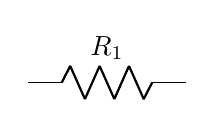
\begin{tikzpicture}
        \draw (0,0) to[R, l=$R_1$] (2,0);
    \end{tikzpicture}

    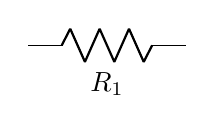
\begin{tikzpicture}
        \draw (0,0) to[R, l_=$R_1$] (2,0);
    \end{tikzpicture}

    When using = or , you must use it inside an \begin{verbatim} \mbox \end{verbatim} command

    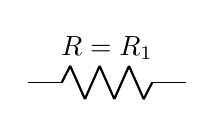
\begin{tikzpicture}
        \draw (0,0) to[R, l=\mbox{$R=R_1$}] (2,0);
    \end{tikzpicture}

    The options that control label orientation are

    \begin{verbatim}
        smartlabels, rotatelabels, straight
    \end{verbatim}

    \section{Current}
    \section{Flow}
    \section{Voltage}

\end{document}
